\documentclass[11pt,a4paper]{article}
% The maths package
\usepackage{amsmath,mathtools,braket,amssymb, amsfonts}
\usepackage{fullpage}
\usepackage{graphicx}
\usepackage{tikz}

% New commands
\newcommand*\tageq{\refstepcounter{equation}\tag{\theequation}}
\newcommand*\circled[1]{\tikz[baseline=(char.base)]{
            \node[shape=circle,draw,inner sep=2pt] (char) {#1};}}

\begin{document}

\begin{titlepage}
\renewcommand{\baselinestretch}{1.0}
\begin{center}

\vspace*{30mm}
\Huge\bf
		Analysis of Steady State Flow in Systems\\
\vspace{20mm}
\large\sl
		by\\
		Ryan Mitchell
		\medskip\\
\rm
\large\sl
		for\\
		MECH2700\\
		Numerical Analysis I\\
\vspace{25mm}
		19 Oct 2015.		
\end{center}
\end{titlepage}


\tableofcontents
\listoffigures
%\listoftables
\newpage

\section{Introduction}
\newpage

\section{A Chebyshev Filter For Electrical Signals}

\medskip	
\begin{figure}[h]
	\centering
	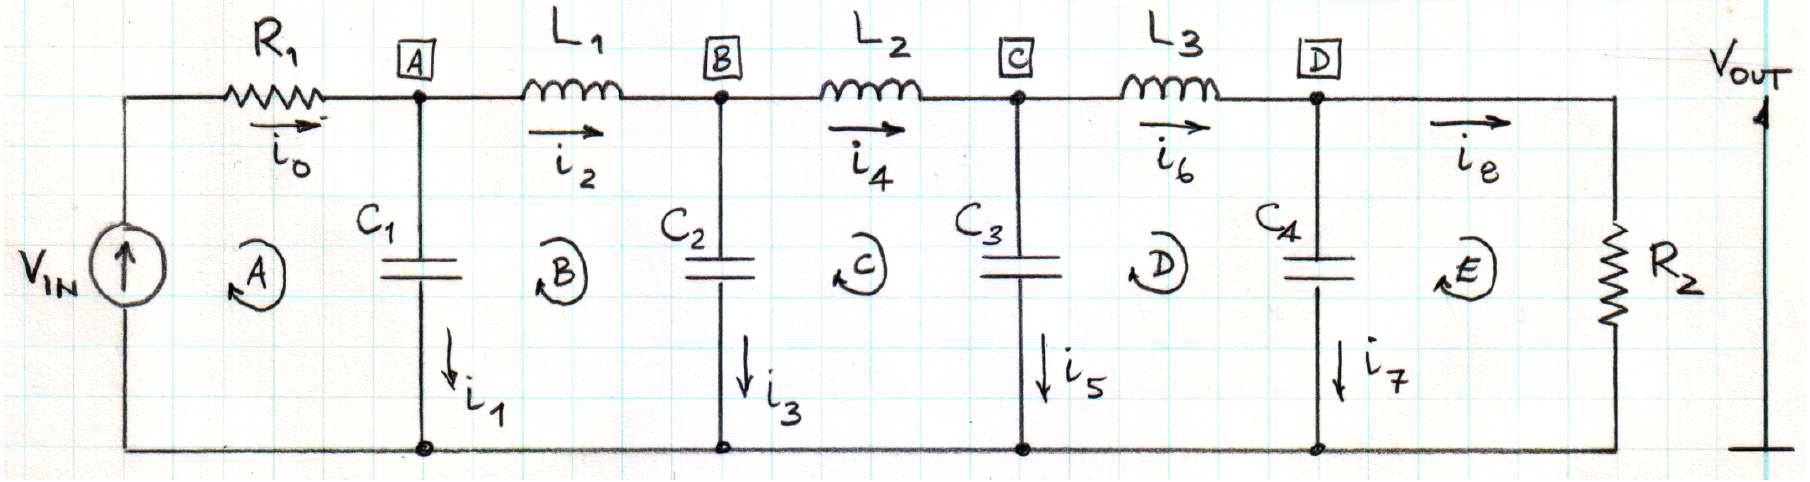
\includegraphics[width=0.9\linewidth]{Images/Circuit.png}
	\caption{Chebyshev Filter Circuit}
	\label{fig:circuit}
\end{figure}

To analyse the circuit provided in Figure \ref{fig:circuit}, Mesh and Nodal Analysis techniques are used. Mesh Analysis is derived from Kirchoff's Voltage Law which states that `the directed sum of the electrical potential differences (voltage) around any closed network is zero'. Nodal Analysis is derived form Kirchoff's Current Law which states that `at any node (junction) in an electrical circuit, the sum of currents flowing into that node is equal to the sum of currents flowing out of that node'. Both tools are required to derive the nine equations in order to solve for the unknowns, $\omega$ and $V_{IN}$, in the system. The five Mesh equations (equations \ref{eq:1} to \ref{eq:5}) and four Node equations (equations \ref{eq:6} to \ref{eq:9}) were found to be

\begin{align}
	&\circled{A} \quad V_{IN} - Z_{R1}i_{0} - Z_{C1}i_{1} = 0 \tageq\label{eq:1}\\
	&\quad \quad \, \, V_{IN} = Z_{R1}i_{0} + Z_{C1}i_{1} \notag \\
	&\circled{B} \quad Z_{C1}i_{1} - Z_{L1}i_{2} - Z_{C2}i_{3} = 0 \tageq\label{eq:2}\\
	&\circled{C} \quad Z_{C2}i_{3} - Z_{L2}i_{4} - Z_{C3}i_{5} = 0 \tageq\label{eq:3}\\
	&\circled{D} \quad Z_{C3}i_{5} - Z_{L3}i_{6} - Z_{C4}i_{7} = 0 \tageq\label{eq:4}\\
	&\circled{E} \quad Z_{C4}i_{7} - Z_{R2}i_{8} = 0 \tageq\label{eq:5}
\end{align}
\begin{align}
	&\boxed{A} \quad i_{0} - i_{1} - i_{2} = 0 \tageq\label{eq:6}\\
	&\boxed{B} \quad i_{2} - i_{3} - i_{4} = 0 \tageq\label{eq:7}\\
	&\boxed{C} \quad i_{4} - i_{5} - i_{6} = 0 \tageq\label{eq:8}\\
	&\boxed{D} \quad i_{6} - i_{7} - i_{8} = 0 \tageq\label{eq:9}
\end{align}\\

These equations can then be compiled into matrix form in order to make use of software tools.\\

$\begin{bmatrix*}
	Z_{R1} & Z_{C1} & 0 & 0 & 0 & 0 & 0 & 0 & 0 \\
	0 & Z_{C1} & -Z_{L1} & -Z_{C2} & 0 & 0 & 0 & 0 & 0\\
	0 & 0 &  0 & Z_{C2} & -Z_{L2} & -Z_{C3} & 0 & 0 & 0\\
	0 & 0 & 0 & 0 & 0 & Z_{C3} & -Z_{L3} & -Z_{C4} & 0\\
	0 & 0 & 0 & 0 & 0 & 0 & 0 & Z_{C4} & -Z_{R2}\\
	1 & -1 & -1 & 0 & 0 & 0 & 0 & 0 & 0\\
	0 & 0 & 1 & -1 & -1 & 0 & 0 & 0 & 0\\
	0 & 0 & 0 & 0 & 1 & -1 & -1 & 0 & 0\\
	0 & 0 & 0 & 0 & 0 & 0 & 1 & -1 & -1\\
\end{bmatrix*}$
$ * $
$\begin{bmatrix}
	i_{0}\\
	i_{1}\\
	i_{2}\\
	i_{3}\\
	i_{4}\\
	i_{5}\\
	i_{6}\\
	i_{7}\\
	i_{8}\\
\end{bmatrix}$
$ = $
$\begin{bmatrix}
	V_{IN}\\
	0\\
	0\\
	0\\
	0\\
	0\\
	0\\
	0\\
	0\\
\end{bmatrix}$ \bigskip

Which becomes \\

$\begin{bmatrix*}
	R_{1} & \frac{-j}{\omega C_{1}} & 0 & 0 & 0 & 0 & 0 & 0 & 0 \\
	0 & \frac{-j}{\omega C_{1}} & -j \omega L_{1} & \frac{j}{\omega C_{2}} & 0 & 0 & 0 & 0 & 0\\
	0 & 0 &  0 & \frac{-j}{\omega C_{2}} & -j \omega L_{2} & \frac{j}{\omega C_{3}} & 0 & 0 & 0\\
	0 & 0 & 0 & 0 & 0 & \frac{-j}{\omega C_{3}} & -j \omega L_{3} & \frac{j}{\omega C_{4}} & 0\\
	0 & 0 & 0 & 0 & 0 & 0 & 0 & \frac{-j}{\omega C_{4}} & -R_{2}\\
	1 & -1 & -1 & 0 & 0 & 0 & 0 & 0 & 0\\
	0 & 0 & 1 & -1 & -1 & 0 & 0 & 0 & 0\\
	0 & 0 & 0 & 0 & 1 & -1 & -1 & 0 & 0\\
	0 & 0 & 0 & 0 & 0 & 0 & 1 & -1 & -1\\
\end{bmatrix*}$
$ * $
$\begin{bmatrix}
	i_{0}\\
	i_{1}\\
	i_{2}\\
	i_{3}\\
	i_{4}\\
	i_{5}\\
	i_{6}\\
	i_{7}\\
	i_{8}\\
\end{bmatrix}$ 
$ = $
$\begin{bmatrix}
	V_{IN}\\
	0\\
	0\\
	0\\
	0\\
	0\\
	0\\
	0\\
	0\\
\end{bmatrix}$

Need to check for singularity of the matrix as the first step of the function!
\newpage

\section{A Water-Supply Network}
\end{document}
